%!TeX root = CSPCL_NTN2026_slides_fr_v2.tex
\documentclass[aspectratio=169,10pt]{beamer}

% ============================== SETUP ==============================
\usepackage{fontspec}
\setmainfont{TeX Gyre Heros}
\setsansfont{TeX Gyre Heros}
\newfontfamily\monofont{Noto Sans Mono}
\usepackage{polyglossia}
\setdefaultlanguage{french}

\usetheme[progressbar=frametitle,numbering=counter,background=light]{metropolis}
\setbeamertemplate{navigation symbols}{}
\setbeamertemplate{frame numbering}[counter]

\usepackage{tikz}
\usetikzlibrary{arrows.meta,positioning,calc,shapes.geometric}
\usepackage{tcolorbox}
\tcbuselibrary{skins}
\usepackage{graphicx}
\usepackage{adjustbox}
\usepackage{pgfpages}
\graphicspath{{slides_assets/}}

% ---- toggle: false = presentation only, true = adds speaker-note pages
\newif\ifshownotes
\shownotesfalse
\ifshownotes
  \setbeameroption{show notes on second screen=right}
\fi

% ============================== PALETTE (light) ==============================
\definecolor{bg}{HTML}{F7F9FC}
\definecolor{bgpanel}{HTML}{EFF3F9}
\definecolor{bgpanel2}{HTML}{E7ECF3}
\definecolor{line}{HTML}{8C9AB0}
\definecolor{linesoft}{HTML}{B4C0D1}
\definecolor{ink}{HTML}{16202E}
\definecolor{inkdim}{HTML}{435166}
\definecolor{inkfaint}{HTML}{7C8CA3}
\definecolor{accent}{HTML}{B8710F}
\definecolor{accenttwo}{HTML}{0E7D6F}
\definecolor{warning}{HTML}{C2464E}
\definecolor{accentinkon}{HTML}{FFF6E9}
\definecolor{accenttwoinkon}{HTML}{EAFBF6}

\setbeamercolor{background canvas}{bg=bg}
\setbeamercolor{normal text}{fg=ink,bg=bg}
\setbeamercolor{frametitle}{fg=ink,bg=bg}
\setbeamercolor{framesubtitle}{fg=inkdim}
\setbeamercolor{progress bar}{fg=accent,bg=linesoft}
\setbeamercolor{title separator}{fg=accent}
\setbeamercolor{alerted text}{fg=warning}
\setbeamercolor{example text}{fg=accenttwo}
\setbeamercolor{page number in head/foot}{fg=inkdim}
\setbeamerfont{page number in head/foot}{family=\monofont,size=\small,series=\bfseries}
\setbeamerfont{frametitle}{series=\bfseries,size=\Large}
\setbeamerfont{framesubtitle}{family=\monofont,size=\scriptsize}
\setbeamertemplate{frametitle continuation}{}

\setbeamertemplate{itemize item}{\textcolor{accenttwo}{\scriptsize$\blacktriangleright$}}
\setbeamertemplate{itemize subitem}{\textcolor{inkdim}{\tiny$-$}}
\setlength{\parskip}{4pt}

% ============================== MACROS ==============================
\newcommand{\muD}{\ensuremath{\mu}D3TN}
\newcommand{\eyebrow}[1]{\textcolor{inkdim}{\small\monofont \MakeUppercase{#1}}}

\newtcbox{\chip}[1][]{on line, arc=9pt, colframe=line, colback=bgpanel2,
  boxrule=0.8pt, top=4pt, bottom=4pt, left=10pt, right=10pt,
  fontupper=\monofont\normalsize, before upper={\color{ink}}, #1}
\newtcbox{\chipstrong}[1][]{on line, arc=9pt, colframe=accent, colback=bgpanel2,
  boxrule=1pt, top=4pt, bottom=4pt, left=10pt, right=10pt,
  fontupper=\monofont\normalsize\bfseries, before upper={\color{ink}}, #1}
\newtcbox{\milestone}[1][]{on line, arc=10pt, colframe=accenttwo, colback=accenttwo,
  boxrule=0pt, top=5pt, bottom=5pt, left=14pt, right=14pt,
  fontupper=\monofont\normalsize\bfseries, before upper={\color{accenttwoinkon}}, #1}

% \bigfig maximizes a tikzpicture to fill the space freed by removing
% titles/prose: it scales up to whichever of width/height is tighter.
\newcommand{\bigfig}[2][0.82\textheight]{\begin{center}\adjustbox{max width=\linewidth,max height=#1}{#2}\end{center}}

% \photo frames a real photo consistently with the vector panels: a thin
% rule border, scaled to fit within the given width/height box.
\newcommand{\photo}[3]{\adjustbox{cfbox=line 1.4pt 0pt,max width=#1,max height=#2}{\includegraphics{#3}}}

\newcommand{\led}[1]{\tikz[baseline=-0.6ex]{\filldraw[#1,draw=#1] (0,0) circle (2.1pt);}}

% simple padlock glyph, centered at (x,y), in the given color
\newcommand{\lockicon}[3]{%
  \draw[#3,fill=#3,rounded corners=2pt] (#1-0.32,#2-0.30) rectangle (#1+0.32,#2+0.22);
  \draw[#3,line width=2.4pt] (#1-0.2,#2+0.22) arc (180:0:0.2);
}

\newtcolorbox{cardbox}{colback=bgpanel2, colframe=line, boxrule=0.6pt,
  arc=6pt, left=14pt, right=14pt, top=7pt, bottom=7pt, coltext=ink}

\tikzset{
  panel/.style={draw=line, line width=1pt, fill=bgpanel, rounded corners=3pt},
  panel2/.style={draw=line, line width=1pt, fill=bgpanel2, rounded corners=3pt},
  accentbox/.style={draw=accent, fill=accent, rounded corners=3pt},
  accenttwobox/.style={draw=accenttwo, fill=accenttwo, rounded corners=3pt},
  warnbox/.style={draw=warning, line width=1.1pt, fill=bgpanel2, rounded corners=3pt},
  arrline/.style={-{Latex[length=2.8mm,width=2mm]}, line width=1.3pt, draw=inkdim},
  accline/.style={-{Latex[length=2.4mm,width=1.7mm]}, line width=1.3pt, draw=accenttwo},
  dimline/.style={line width=0.9pt, draw=inkdim, dash pattern=on 3pt off 3pt},
  lbl/.style={font=\monofont\normalsize, text=inkdim},
  lblf/.style={font=\monofont\normalsize, text=inkdim},
  lbli/.style={font=\monofont\normalsize, text=ink},
  lbld/.style={font=\bfseries\sffamily\Large, text=ink},
}

% one-line explanatory caption under a figure (review: "un peu plus de texte")
\newcommand{\takeaway}[1]{{\normalsize\color{inkdim} #1}}

% overview card: title + list of items
\newcommand{\ovcard}[2]{%
  \begin{tcolorbox}[colback=bgpanel2, colframe=line, boxrule=0.6pt, arc=6pt,
    left=8pt, right=8pt, top=4pt, bottom=5pt, coltext=ink, height=0.37\textheight, valign=top]
  {\small\monofont\bfseries\color{accent}\MakeUppercase{#1}}\par\vspace{2pt}
  {\small\raggedright #2\par}
  \end{tcolorbox}}
\newtcolorbox{smallcard}[1]{colback=bgpanel2, colframe=line, boxrule=0.6pt, arc=6pt,
  left=6pt, right=6pt, top=6pt, bottom=6pt, coltext=ink, equal height group=#1}
\newcommand{\nowled}{\led{accenttwo}\ }
\newcommand{\laterled}{\led{linesoft}\ }

% one protocol stack (GIF style): \stack{x}{title}{list of layer/style pairs, bottom first}
% each layer is 1.6 wide x 0.62 high
\newcommand{\layer}[4]{% x, y, style, label
  \draw[#3] (#1,#2) rectangle ++(2.2,0.62);
  \node[font=\monofont\small,text=ink] at (#1+1.1,#2+0.31) {#4};}
\tikzset{
  lyr/.style={draw=line, line width=0.9pt, fill=bgpanel},
  lyrbus/.style={draw=line, line width=0.9pt, fill=bgpanel2},
  lyrbp/.style={draw=accenttwo, line width=0.9pt, fill=accenttwo!25},
  lyrcl/.style={draw=accent, line width=0.9pt, fill=accent!30},
}

\title{Adoption progressive des DTN pour les opérateurs de CubeSats}
\author{Sarah Theoulle, Olivier De Jonck\`ere}
\date{NTN Days 2026}
\hypersetup{pdftitle={Adoption progressive des DTN pour les opérateurs de CubeSats --- NTN Days 2026},pdfauthor={Sarah Theoulle, Olivier De Jonck\`ere}}

\begin{document}

% ============================== TITLE ==============================
\begin{frame}[plain]
\vspace{2pt}

\eyebrow{NTN Days 2026 - Paris, France}\\[14pt]
{\fontsize{24}{29}\selectfont\bfseries\color{ink} Adoption progressive des DTN\\ pour les opérateurs de CubeSats}\\[20pt]

\chip{Sarah Theoulle} \chip{Olivier De Jonck\`ere}

\vspace{8pt}
\chip{LIRMM $\cdot$ CSUM}

\vfill
\begin{tikzpicture}[baseline=0pt]
  \foreach \x/\w in {0.4/2.2,2.9/1.4,4.6/2.8,7.7/0.9,8.9/1.9,11.1/1.1,12.5/2.3}
    \fill[accenttwo] (\x,0) rectangle ++(\w,0.22);
  \fill[accent] (9.9,0) rectangle ++(0.55,0.22);
  \draw[inkdim,line width=0.5pt] (0,-0.14) -- (15.2,-0.14);
\end{tikzpicture}

\note{Bonjour. Je vais vous présenter comment amener progressivement les réseaux tolérants aux délais chez les opérateurs de CubeSats qui utilisent déjà le CubeSat Space Protocol, sans toucher à ce qui fonctionne déjà. C'est un travail du LIRMM, mené avec le Centre Spatial Universitaire de Montpellier, et une partie d'un projet plus large.}
\end{frame}

% ============================== OVERVIEW (VISTA) ==============================
\begin{frame}{Le projet VISTA}

\vfill
\begin{columns}[T]
\begin{column}{0.49\textwidth}
\ovcard{Outillage}{%
\nowled Protocole --- BP + CSPCL\\
\nowled Routage --- A-SABR\\
\nowled Interopérabilité --- Charon}
\end{column}
\begin{column}{0.49\textwidth}
\ovcard{Modèles}{%
\laterled Optimisation du routage\\
\laterled Internetworking}
\end{column}
\end{columns}

\vspace{4pt}
\begin{columns}[T]
\begin{column}{0.49\textwidth}
\ovcard{Ambitions}{%
\laterled Un vrai réseau DTN pour les opérations\\
\laterled BP + routage sur microcontrôleur\\
\laterled Un laboratoire pour les chercheurs}
\end{column}
\begin{column}{0.49\textwidth}
\ovcard{Partenaires}{%
\laterled CSUM\\
\laterled Étudiants de Montpellier et d'ailleurs\\
\laterled INRIA, D3TN, Université de Bologne \dots}
\end{column}
\end{columns}

\note{CSPCL et Charon font partie d'un projet plus large, VISTA. Côté outillage : le protocole, avec Bundle Protocol et CSPCL ; le routage, avec A-SABR ; et l'interopérabilité, avec Charon. Côté modèles : l'optimisation du routage et l'internetworking. Nos ambitions : un vrai réseau DTN pour les opérations, le protocole et le routage sur microcontrôleur, et un laboratoire pour les chercheurs. Et tout cela avec nos partenaires : le CSUM, les étudiants de Montpellier et d'ailleurs, l'INRIA, D3TN et l'Université de Bologne. Aujourd'hui, je parle des briques d'outillage.}
\end{frame}

% ============================== CSUM (building + control room) ==============================
\begin{frame}{Le CSUM}

\vfill
\centering
\begin{columns}[c]
\begin{column}{0.42\textwidth}\centering
\photo{\linewidth}{0.55\textheight}{csum_building.png}
\end{column}
\begin{column}{0.54\textwidth}\centering
\photo{\linewidth}{0.55\textheight}{control_room.png}
\end{column}
\end{columns}

\vspace{12pt}
\chip{Montpellier, France}\\[8pt]
\takeaway{Centre Spatial Universitaire de Montpellier: de vraies opérations en vol,\\ une mission CubeSat 12U en préparation.}
\vfill

\note{Ce travail existe grâce à un vrai client : le CSUM, le Centre Spatial Universitaire de Montpellier. À droite, sa salle de contrôle : de vraies opérations, menées par une petite équipe, sur une pile qu'elle connaît par cœur. Le CSUM prépare une mission CubeSat 12U et, comme la plupart des équipes CubeSat universitaires, il fonctionne avec un petit budget. On ne remplace pas une telle pile du jour au lendemain : c'est la réalité que toute transition vers le DTN doit respecter.}
\end{frame}

% ============================== DTN (GIF frames 1-2) ==============================
\begin{frame}{Les DTN}

\vfill
\centering
\includegraphics<1>[width=\linewidth,height=0.6\textheight,keepaspectratio]{dtn_gif_1.png}%
\includegraphics<2>[width=\linewidth,height=0.6\textheight,keepaspectratio]{dtn_gif_2.png}

\vspace{8pt}
\takeaway{Stocker, transporter, retransmettre : un nœud garde le \emph{bundle} jusqu'au prochain contact.}\\[4pt]
{\small\color{inkdim} Architecture DTN : RFC 4838 \quad$\cdot$\quad Bundle Protocol v7 : RFC 9171}
\vfill

\note{Les réseaux tolérants aux délais, définis par l'architecture de la RFC 4838. Le protocole standard est Bundle Protocol, version 7, RFC 9171 : l'unité de données est le bundle. Prenons un rover sur Mars qui veut joindre un opérateur sur Terre. Il transmet son bundle à un orbiteur au moment d'un contact. [clic] L'orbiteur n'a pas encore de lien vers la Terre : il garde le bundle en stockage, et le transporte avec lui sur son orbite.}
\end{frame}

% ============================== DTN (GIF frames 3-4) ==============================
\begin{frame}{Les DTN --- un protocole overlay}

\vfill
\centering
\includegraphics<1>[width=\linewidth,height=0.6\textheight,keepaspectratio]{dtn_gif_3.png}%
\includegraphics<2>[width=\linewidth,height=0.6\textheight,keepaspectratio]{dtn_gif_4.png}

\vspace{8pt}
\takeaway{Longs délais, longues interruptions : pas besoin d'un chemin de bout en bout permanent.}\\[4pt]
{\small\color{inkdim} BP est un \textbf{protocole overlay} : il se pose sur n'importe quel transport, via un CLA.}
\vfill

\note{Au contact suivant, l'orbiteur retransmet le bundle vers la station sol, malgré la distance interplanétaire et le long délai. [clic] La station le remet ensuite à l'opérateur, cette fois sur l'Internet classique. Regardez la pile de la station : BP se pose aussi bien au-dessus d'un lien spatial que d'une pile TCP/IP. C'est un protocole overlay : il s'adapte à n'importe quel transport, grâce à un adaptateur de couche de convergence, un CLA.}
\end{frame}

% ============================== WHY BP ==============================
\begin{frame}{Pourquoi BP ?}

\vfill
\centering{\Large\color{ink}\bfseries Un protocole d'avenir.}\\[6pt]
\takeaway{Conçu pour les futures missions d'exploration spatiale\\ et pour le futur \emph{Solar System Internet}.}

\vspace{14pt}
\begin{columns}[T]
\begin{column}{0.32\textwidth}
\begin{smallcard}{std}\centering
{\bfseries IETF}\\[3pt]
{\small\color{inkdim} standardise Bundle Protocol v7 (RFC 9171)}
\end{smallcard}
\end{column}
\begin{column}{0.32\textwidth}
\begin{smallcard}{std}\centering
{\bfseries CCSDS}\\[3pt]
{\small\color{inkdim} normalise BP pour les communications spatiales}
\end{smallcard}
\end{column}
\begin{column}{0.32\textwidth}
\begin{smallcard}{std}\centering
{\bfseries IOAG}\\[3pt]
{\small\color{inkdim} en fait la base du \emph{Solar System Internet}}
\end{smallcard}
\end{column}
\end{columns}

\vspace{12pt}
{\small\color{inkdim} Déjà au cœur des futures architectures}\\[6pt]
\chip{NASA LCRNS} \chip{ESA Moonlight} \chip{NASA–ESA LunaNet}
\vfill

\note{Pourquoi Bundle Protocol plutôt qu'autre chose ? Parce que c'est un protocole d'avenir : il est prévu pour les futures missions d'exploration spatiale, et pour le futur Solar System Internet. Les efforts de standardisation convergent : l'IETF a standardisé BP version 7 avec la RFC 9171, le CCSDS le normalise pour les communications spatiales, et l'IOAG en fait la base du Solar System Internet. On le retrouve déjà au cœur des futures architectures lunaires : LCRNS à la NASA, Moonlight à l'ESA, et LunaNet, porté par la NASA et l'ESA.}
\end{frame}

% ============================== CHALLENGE 1 ==============================
\begin{frame}{Le challenge}

\vfill
\centering{\Large\color{ink}\bfseries Comment introduire les DTN sans être intrusif ?}

\vspace{10pt}
\begin{columns}[T]
\begin{column}{0.32\textwidth}
\begin{smallcard}{chal}\centering
{\bfseries CSP, éprouvé en vol}\\[3pt]
{\small\color{inkdim} réseau interne du satellite, très répandu chez les CubeSats --- mais pas DTN}
\end{smallcard}
\end{column}
\begin{column}{0.32\textwidth}
\begin{smallcard}{chal}\centering
{\bfseries BP, séduisant\dots}\\[3pt]
{\small\color{inkdim} \dots\ mais changer de pile est un risque, et toutes les applications ne parlent pas BP}
\end{smallcard}
\end{column}
\begin{column}{0.32\textwidth}
\begin{smallcard}{chal}\centering
{\bfseries Les petits acteurs}\\[3pt]
{\small\color{inkdim} ne sont pas prêts à faire le saut sans en avoir évalué les gains}
\end{smallcard}
\end{column}
\end{columns}

\vspace{10pt}
\begin{cardbox}\centering
\led{accenttwo}\ \textbf{Notre levier :} BP est un overlay --- on peut le poser \emph{sur} CSP,\\ et tester la tolérance aux délais \textbf{sans changer la pile}.
\end{cardbox}
\vfill

\note{Voici le challenge: Les opérateurs de CubeSats utilisent CSP, le CubeSat Space Protocol : il a fait ses preuves en vol comme réseau interne du satellite, et il est largement utilisé dans la communauté CubeSat. Mais ce n'est pas un protocole DTN. Bundle Protocol est séduisant\dots\ mais passer de CSP à BP, c'est changer toute la pile : un risque que les petits acteurs ne sont pas prêts à prendre avant d'en avoir évalué les gains. Et au-delà du risque sur le protocole, toutes les applications ne parlent pas BP. Notre levier, c'est la nature overlay de BP : on peut le faire tourner au-dessus de CSP, et proposer aux opérateurs de tester la tolérance aux délais sans changer leur pile.}
\end{frame}

% ============================== CSPCL: BRICK IN THE STACK ==============================
\begin{frame}{CSPCL}

\vfill
\bigfig[0.56\textheight]{\begin{tikzpicture}
% node A
\node[font=\monofont\small\bfseries,text=ink] at (1.1,4.25) {Nœud DTN A};
\layer{0}{3.1}{lyr}{Application}
\layer{0}{2.48}{lyrbp}{BP}
\layer{0}{1.86}{lyrcl}{CSPCL}
\layer{0}{1.24}{lyr}{CSP}
\layer{0}{0.62}{lyrbus}{CAN}
% CSP-only subsystem
\node[font=\monofont\small\bfseries,text=ink] at (5.1,3.0) {Sous-système CSP};
\layer{4}{1.86}{lyr}{Application}
\layer{4}{1.24}{lyr}{CSP}
\layer{4}{0.62}{lyrbus}{CAN}
% node B
\node[font=\monofont\small\bfseries,text=ink] at (9.1,4.25) {Nœud DTN B};
\layer{8}{3.1}{lyr}{Application}
\layer{8}{2.48}{lyrbp}{BP}
\layer{8}{1.86}{lyrcl}{CSPCL}
\layer{8}{1.24}{lyr}{CSP}
\layer{8}{0.62}{lyrbus}{CAN}
% shared CAN bus
\draw[accenttwo,line width=2.2pt] (-0.3,0.1) -- (10.5,0.1);
\foreach \x in {1.1,5.1,9.1} \draw[accenttwo,line width=1.2pt] (\x,0.1) -- (\x,0.62);
\node[font=\monofont\small,text=accenttwo,anchor=west] at (10.6,0.1) {bus CAN};
% bundle path
\draw[accline,dashed] (2.0,2.79) -- (2.0,0.35) -- (8.2,0.35) -- (8.2,2.79);
\end{tikzpicture}}

\vspace{8pt}
\centering{\Large\color{ink}\bfseries Un petit adaptateur entre BP et CSP.}\\[6pt]
\takeaway{CSPCL est le CLA qui manquait --- et CSP reste le réseau interne, sur le bus CAN.}
\vfill

\note{Pour poser BP sur CSP, il manquait une petite brique : un adaptateur de couche de convergence entre BP et CSP. Nous l'avons créé : c'est CSPCL. Il prend la place du CLA dans la pile que l'on vient de voir. Et CSP n'est pas remplacé : il reste le réseau interne du satellite, sur le même bus CAN. Les sous-systèmes uniquement CSP continuent de fonctionner à côté, sans rien changer.}
\end{frame}

% ============================== LEVEL 1: TALKING CSP ==============================
\begin{frame}{Niveau 1 : dialoguer avec CSP}

\vfill
\begin{columns}[c]
\begin{column}{0.4\textwidth}\centering
\bigfig[0.66\textheight]{\begin{tikzpicture}
\draw[panel,line width=1.4pt] (0,7.7) rectangle (5,8.7); \node[lbli] at (2.5,8.2) {BPA};
\draw[arrline] (2.5,7.7) -- (2.5,7.2);
\draw[accentbox] (0,6.4) rectangle (5,7.2); \node[font=\monofont\normalsize,text=accentinkon] at (2.5,6.8) {CSPCL};
\draw[arrline] (2.5,6.4) -- (2.5,5.9);
\draw[panel,line width=1.4pt] (0,4.7) rectangle (5,5.9); \node[lbli] at (2.5,5.55) {libcsp};
\node[font=\monofont\normalsize,text=inkdim] at (2.5,5.05) {RDP + SFP};
\draw[arrline] (2.5,4.7) -- (2.5,4.2);
\draw[panel,line width=1.4pt] (0,3.4) rectangle (5,4.2); \node[lbli] at (2.5,3.8) {SocketCAN};
\draw[arrline] (2.5,3.4) -- (2.5,2.9);
\draw[accenttwobox] (0,2.1) rectangle (5,2.9); \node[font=\monofont\normalsize,text=accenttwoinkon] at (2.5,2.5) {BUS CAN};
\end{tikzpicture}}
\end{column}
\begin{column}{0.54\textwidth}
\begin{itemize}
\item \textbf{RDP} : connexions CSP acquittées.
\item \textbf{SFP} : fragmentation, car un bundle dépasse presque toujours la MTU CSP.
\item \textbf{SocketCAN} : le vrai bus CAN, sans matériel en plus.
\end{itemize}

\vspace{8pt}
\takeaway{Ce que TCPCL fait pour TCP, CSPCL le fait pour CSP.}\\[6pt]
{\small\color{inkdim} BP étant un protocole overlay, autant profiter des technologies d'Internet (TCPCL) pour la partie du réseau DTN qui recouvre Internet.}
\end{column}
\end{columns}
\vfill

\note{Premier niveau : dialoguer avec CSP. Le rôle d'un adaptateur de couche de convergence est de faire correspondre la transmission de bundles à un transport sous-jacent, comme TCPCL le fait pour TCP. CSPCL s'appuie sur deux fonctionnalités de CSP : RDP pour les connexions acquittées, et SFP pour la fragmentation, car un bundle est presque toujours plus gros que la MTU d'un paquet CSP. Et il utilise le bus CAN via SocketCAN : les bundles empruntent exactement le même câble que le reste du satellite. Et comme BP est un protocole overlay, on garde TCPCL là où le réseau DTN recouvre Internet : c'est exactement ce qu'on a vu avec la station sol tout à l'heure.}
\end{frame}

% ============================== LEVEL 2: RELIABILITY ==============================
\begin{frame}{Niveau 2 : fiabilité des bundles sur CSP}

\vfill
\begin{columns}[c]
\begin{column}{0.52\textwidth}\centering
\bigfig[0.66\textheight]{\begin{tikzpicture}
\node[lbli] at (0.8,7.1) {ÉMETTEUR}; \node[lbli] at (7.5,7.1) {RÉCEPTEUR};
\draw[dimline] (0.8,0.2) -- (0.8,6.8);
\draw[dimline] (7.5,0.2) -- (7.5,6.8);
\draw[arrline] (0.8,6.2) -- (7.5,6.2); \node[lblf] at (4.15,6.45) {morceau 1 du bundle};
\draw[arrline] (0.8,5.5) -- (7.5,5.5); \node[lblf] at (4.15,5.75) {morceau N du bundle};
\draw[accline] (7.5,4.7) -- (0.8,4.7);
\node[font=\monofont\normalsize,text=accenttwo] at (4.15,5.0) {ACK : bundle réassemblé};
\draw[panel2] (0.4,2.4) rectangle (7.9,4.2);
\node[lbl] at (4.15,3.85) {pas d'ACK à temps};
\node[font=\monofont\normalsize,text=accent] at (4.15,3.35) {un seul nouvel essai};
\node[font=\monofont\normalsize,text=warning] at (4.15,2.85) {échec : on prévient le BPA};
\end{tikzpicture}}

\takeaway{\small Un ACK de bout en bout, propre à CSPCL.}
\end{column}
\begin{column}{0.44\textwidth}\centering
\bigfig[0.6\textheight]{\begin{tikzpicture}
\draw[panel,line width=1.4pt] (0,3.6) rectangle (3.6,5.3); \node[font=\sffamily\bfseries,text=ink] at (1.8,4.45) {Unibo-BP};
\draw[panel,line width=1.4pt] (5.2,3.6) rectangle (8.8,5.3); \node[font=\sffamily\bfseries,text=ink] at (7.0,4.45) {\muD};
\draw[panel,line width=1.4pt] (10.4,3.6) rectangle (14.0,5.3); \node[font=\sffamily\bfseries,text=ink] at (12.2,4.45) {Hardy};
\draw[arrline] (1.8,3.6) -- (1.8,2.5);
\draw[arrline] (7.0,3.6) -- (7.0,2.1);
\draw[arrline] (12.2,3.6) -- (12.2,2.5);
\draw[line,line width=1.2pt] (1.8,2.5) -- (12.2,2.5);
\draw[accentbox] (4.3,1.2) rectangle (9.7,2.1);
\node[font=\monofont\normalsize,text=accentinkon] at (7.0,1.65) {libcspcl};
\end{tikzpicture}}

\takeaway{\small 3 implémentations différentes\\ du Bundle Protocol, un même cœur.}
\end{column}
\end{columns}
\vfill

\note{Deuxième niveau : la fiabilité des bundles sur CSP. Un bundle est découpé en plusieurs morceaux pour passer sur CSP. Or les acquittements de CSP confirment seulement qu'un paquet a été transmis, pas que l'autre extrémité a réassemblé tout le bundle. CSPCL ajoute donc son propre acquittement de bout en bout, fait un seul nouvel essai, et prévient le BPA en cas d'échec persistant. Et c'est portable : le même cœur est intégré dans trois implémentations différentes du Bundle Protocol --- Unibo-BP en démon autonome, µD3TN dans le même processus, Hardy via une liaison FFI Rust asynchrone.}
\end{frame}

% ============================== CHALLENGE 2 ==============================
\begin{frame}{Challenge 2}

\vfill
\bigfig[0.42\textheight]{\begin{tikzpicture}
\draw[panel,line width=1.4pt] (0,4.9) rectangle (4.3,6.3); \node[lbli] at (2.15,5.6) {APPLICATION CSP};
\lockicon{2.15}{4.55}{accent}
\node[lbl,text=accent,anchor=west] at (4.8,4.55) {AU-DESSUS : ?};
\draw[accenttwobox] (0,2.7) rectangle (4.3,4.1); \node[font=\monofont\normalsize\bfseries,text=accenttwoinkon] at (2.15,3.4) {BP};
\lockicon{2.15}{2.35}{accenttwo}
\node[lbl,text=accenttwo,anchor=west] at (4.8,2.35) {EN DESSOUS : CSPCL};
\draw[panel,line width=1.4pt] (0,0.5) rectangle (4.3,1.9); \node[lbli] at (2.15,1.2) {CSP / BUS CAN};
\end{tikzpicture}}

\vspace{10pt}
\centering{\Large\color{ink}\bfseries Comment les applications existantes\\ peuvent-elles devenir tolérantes aux délais ?}\\[8pt]
\takeaway{Elles volent déjà, sont qualifiées, et parlent CSP : pas question de les réécrire.}
\vfill

\note{BP circule maintenant sur CSP. Mais il reste un second challenge : les applications. Elles volent déjà, elles sont qualifiées, et elles parlent du CSP pur. Comment peuvent-elles profiter de la tolérance aux délais, sans être réécrites pour parler Bundle Protocol ?}
\end{frame}

% ============================== CHARON (merged) ==============================
\begin{frame}{Charon}

\vfill
\bigfig[0.36\textheight]{\begin{tikzpicture}[font=\monofont\normalsize]
\draw[panel,line width=1.4pt] (0,1.2) rectangle (1.9,2.2); \node[lbli] at (0.95,1.7) {Alice};
\draw[accenttwobox] (2.5,1.05) rectangle (4.9,2.35); \node[text=accenttwoinkon] at (3.7,1.7) {Charon};
\draw[panel,line width=1.4pt] (5.5,1.2) rectangle (8.4,2.2); \node[lbli] at (6.95,1.7) {BPA d'Alice};
\draw[panel2] (9.0,1.2) rectangle (11.9,2.2); \node[text=inkdim] at (10.45,1.7) {topologie DTN};
\draw[panel,line width=1.4pt] (12.5,1.2) rectangle (15.4,2.2); \node[lbli] at (13.95,1.7) {BPA de Bob};
\draw[accenttwobox] (16.0,1.05) rectangle (18.4,2.35); \node[text=accenttwoinkon] at (17.2,1.7) {Charon};
\draw[panel,line width=1.4pt] (19.0,1.2) rectangle (20.9,2.2); \node[lbli] at (19.95,1.7) {Bob};

\draw[arrline] (1.9,1.7) -- (2.4,1.7); \draw[arrline] (4.9,1.7) -- (5.4,1.7);
\draw[arrline] (8.4,1.7) -- (8.9,1.7); \draw[arrline] (11.9,1.7) -- (12.4,1.7);
\draw[arrline] (15.4,1.7) -- (15.9,1.7); \draw[arrline] (18.4,1.7) -- (18.9,1.7);

\node[text=inkdim] at (2.15,2.55) {CSP}; \node[text=inkdim] at (5.15,2.55) {AAP2};
\node[text=inkdim] at (8.65,2.55) {bundle}; \node[text=inkdim] at (12.15,2.55) {bundle};
\node[text=inkdim] at (15.65,2.55) {AAP2}; \node[text=inkdim] at (18.65,2.55) {CSP};
\end{tikzpicture}}

\vspace{10pt}
\centering{\Large\color{ink}\bfseries Un proxy : les paquets CSP, emballés dans des bundles.}\\[8pt]
\takeaway{À l'arrivée, Charon les redescend en CSP ordinaire.}\\[4pt]
\takeaway{Ni Alice ni Bob n'ont changé une ligne de code.}
\vfill

\note{Notre réponse au second challenge, c'est Charon. C'est un proxy léger, placé à côté d'une application CSP. L'application d'Alice parle du CSP pur à son instance locale de Charon, qui emballe ces paquets CSP dans des bundles et les confie à son BPA, ici via l'interface AAP2 de µD3TN. Le bundle traverse la topologie DTN, en profitant du stockage et de la retransmission. De l'autre côté, le BPA de Bob le remet à son Charon, qui le redescend en CSP ordinaire vers Bob. Aucune des deux applications n'a changé. Avec CSPCL en dessous et Charon au-dessus, on a tout le sandwich : CSP, BP, CSP.}
\end{frame}

% ============================== HOW WE TEST ==============================
\begin{frame}{Comment on teste}

\vfill
\centering{\Large\color{ink}\bfseries On a toutes les briques. Comment les valider ?}

\vspace{16pt}
\begin{columns}[T]
\begin{column}{0.32\textwidth}
\begin{smallcard}{test}\centering
{\bfseries Une chaîne complète}\\[3pt]
{\small\color{inkdim} hétérogène, de bout en bout}
\end{smallcard}
\end{column}
\begin{column}{0.32\textwidth}
\begin{smallcard}{test}\centering
{\bfseries Un routage réaliste}\\[3pt]
{\small\color{inkdim} avec la bibliothèque A-SABR}
\end{smallcard}
\end{column}
\begin{column}{0.32\textwidth}
\begin{smallcard}{test}\centering
{\bfseries Du vrai matériel}\\[3pt]
{\small\color{inkdim} et des coupures provoquées}
\end{smallcard}
\end{column}
\end{columns}
\vfill

\note{Nous avons maintenant toutes les briques : CSPCL en dessous, Charon au-dessus. Comment les valider ? Avec trois ingrédients : une chaîne complète et hétérogène, un routage réaliste grâce à A-SABR, et du vrai matériel, sur lequel on provoque des coupures.}
\end{frame}

% ============================== FOUR-NODE CHAIN ==============================
\begin{frame}{À quoi ressemble la chaîne complète}

\vfill
\bigfig[0.62\textheight]{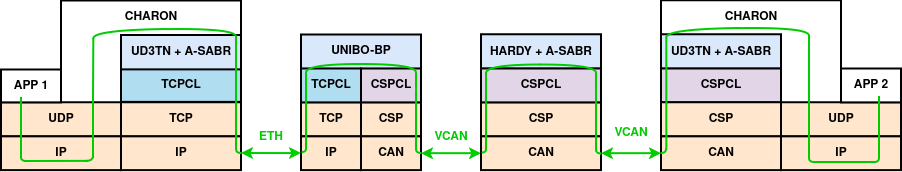
\includegraphics{full_chain.png}}

\vspace{6pt}
\centering\takeaway{4 nœuds, 3 implémentations de BP, 3 transports : validation par un test d'interopérabilité.}
\vfill

\note{Voici la chaîne de test : quatre nœuds, où chaque saut utilise volontairement une combinaison transport et implémentation BP différente --- c'est un test d'interopérabilité. Alice est un µD3TN avec le routage A-SABR, qui fait entrer du trafic via Charon et le fait sortir en TCPCL. Unibo-BP le reçoit en TCPCL et le transmet sur un bus CAN via CSPCL. Hardy, avec A-SABR, parle CAN des deux côtés. Et le tout arrive chez Bob, de nouveau µD3TN, qui le rend à Charon puis à l'application réceptrice.}
\end{frame}

% ============================== A-SABR ==============================
\begin{frame}{Adaptive library for Schedule-Aware Bundle Routing (A-SABR)}

\vfill
\centering{\Large\color{ink}\bfseries Une bibliothèque pour instancier\\ différentes stratégies de routage.}

\vspace{14pt}
\begin{columns}[T]
\begin{column}{0.48\textwidth}
\begin{itemize}
\item Gestion du volume
\item Ressources des nœuds
\item Support de l'internetworking
\end{itemize}
\end{column}
\begin{column}{0.48\textwidth}
\begin{itemize}
\item Support microcontrôleur
\item Plusieurs backends, pour de nombreux algorithmes différents
\end{itemize}
\end{column}
\end{columns}

\vspace{12pt}
\takeaway{Pas de qualité de service réactive en DTN : la gestion des ressources passe\\ par l'optimisation du routage.}
\vfill

\note{Le routage est assuré par A-SABR, Adaptive library for Schedule-Aware Bundle Routing : une bibliothèque qui permet d'instancier différentes stratégies de routage. Elle est déjà utilisée par d'autres équipes, et elle porte beaucoup de travaux sur la gestion des ressources. En DTN, on ne peut pas faire de qualité de service de manière réactive : il faut l'anticiper, et donc optimiser le routage. A-SABR gère le volume, les ressources des nœuds, l'internetworking, le support microcontrôleur, et propose plusieurs backends pour de nombreux algorithmes.}
\end{frame}

% ============================== TESTBED ==============================
\begin{frame}{Le banc d'essai}

\vfill
\bigfig[0.27\textheight]{\begin{tikzpicture}
\draw[panel,line width=1.4pt] (0,0) rectangle (5,2.2); \node[font=\sffamily\bfseries,text=ink] at (2.5,1.5) {PolarFire SoC};
\node[lbl] at (2.5,0.9) {RISC-V, carte A};
\draw[panel,line width=1.4pt] (10.6,0) rectangle (15.6,2.2); \node[font=\sffamily\bfseries,text=ink] at (13.1,1.5) {PolarFire SoC};
\node[lbl] at (13.1,0.9) {RISC-V, carte B};
\draw[accline,line width=1.6pt] (5,1.1) -- (10.6,1.1);
\foreach \x in {6.4,7.4,8.4,9.2} \draw[line] (\x,1.1) -- (\x,0.55);
\node[font=\monofont\normalsize,text=accenttwo] at (7.8,1.8) {bus CAN (SocketCAN)};
\end{tikzpicture}}

\vspace{8pt}
\begin{columns}[c]
\begin{column}{0.38\textwidth}\centering
\photo{\linewidth}{0.27\textheight}{polarfire_boards.png}
\end{column}
\begin{column}{0.58\textwidth}
\begin{itemize}
\item \textbf{Test de coupure} : un nœud tué en plein transfert --- les bundles sont conservés, puis livrés au redémarrage.
\end{itemize}
\end{column}
\end{columns}

\vspace{8pt}
\centering\takeaway{Pourquoi PolarFire SoC : RISC-V sous Linux, représentatif de l'avionique\\ de la mission 12U du CSUM.}
\vfill

\note{Nous ne nous sommes pas contentés de la simulation. Deux cartes de développement RISC-V Microchip PolarFire SoC, reliées par un vrai bus CAN avec SocketCAN. Pourquoi PolarFire SoC ? Parce que c'est du RISC-V sous Linux, représentatif de l'avionique de la future mission 12U du CSUM. Et nous avons volontairement cassé le système : un nœud tué en plein transfert. Les bundles en transit ont simplement été conservés par le voisin, puis livrés dès le redémarrage, sans perte : le principe DTN du début, en action.}
\end{frame}

% ============================== NEXT STEPS (limitations) ==============================


% ============================== FUTURE WORK ==============================
\begin{frame}{Perspectives}

\vfill
\begin{columns}[T]
\begin{column}{0.32\textwidth}
\begin{smallcard}{fut}\centering
{\bfseries Un modèle d'optimisation}\\[3pt]
{\small\color{inkdim} pour obtenir les limites théoriques du routage, et servir de référence aux benchmarks}
\end{smallcard}
\end{column}
\begin{column}{0.32\textwidth}
\begin{smallcard}{fut}\centering
{\bfseries D3TN cloud-native spatial}\\[3pt]
{\small\color{inkdim} un PCB dédié pour lancer des expériences conteneurisées tolérantes aux délais}
\end{smallcard}
\end{column}
\begin{column}{0.32\textwidth}
\begin{smallcard}{fut}\centering
{\bfseries Un laboratoire volant}\\[3pt]
{\small\color{inkdim} pour les expériences des chercheurs, DTN ou non}
\end{smallcard}
\end{column}
\end{columns}

\vspace{16pt}
\centering\takeaway{CSPCL et Charon ne sont que les premières briques du projet VISTA.}
\vfill

\note{Et au-delà, le projet VISTA prépare plusieurs choses. Un modèle d'optimisation, pour obtenir les limites théoriques du routage et servir de référence aux benchmarks. Une approche cloud-native spatiale autour de D3TN, avec un PCB dédié qui permettra aux chercheurs de lancer des expériences conteneurisées tolérantes aux délais. Et, à terme, un véritable laboratoire volant, pour des expériences DTN comme non DTN.}
\end{frame}

% ============================== ACKNOWLEDGEMENTS ==============================
\begin{frame}{Remerciements}

\vfill
\centering
\photo{0.62\linewidth}{0.55\textheight}{stint.jpg}

\vspace{10pt}
\takeaway{Merci à toutes les personnes qui ont contribué au projet --- dont de nombreux étudiants.}\\[8pt]
\chip{Open source, contributions bienvenues : github.com/DTN-MTP}
\vfill

\note{Ce projet est le fruit d'un travail collectif : merci à toutes les personnes qui y ont contribué, dont beaucoup d'étudiants --- ici, une partie de l'équipe au workshop STINT. Tout est open source, sur GitHub, dans l'organisation DTN-MTP : les contributions sont les bienvenues.}
\end{frame}

% ============================== THANK YOU ==============================
\begin{frame}[plain]
\vspace{18pt}
\eyebrow{Merci}\\[16pt]
{\fontsize{44}{44}\selectfont\bfseries\color{ink} Des questions ?}\\[16pt]
{\Large\color{inkdim} Adoption progressive des DTN\\ pour les opérateurs de CubeSats}\\[16pt]

\chip{Sarah Theoulle} \chip{Olivier De Jonck\`ere}

\vspace{8pt}
\chip{LIRMM $\cdot$ CSUM} \chip{github.com/DTN-MTP}

\note{Merci --- je répondrai volontiers à vos questions, que ce soit sur CSPCL, sur Charon, sur le banc d'essai ou sur le reste du projet VISTA.}
\end{frame}

\end{document}
